\documentclass{standalone}
\usepackage{tikz}
\usetikzlibrary{patterns, positioning}
\usepackage[sfdefault]{ClearSans} %% option 'sfdefault' activates Clear Sans as the default text font
\usepackage[T1]{fontenc}

\begin{document}
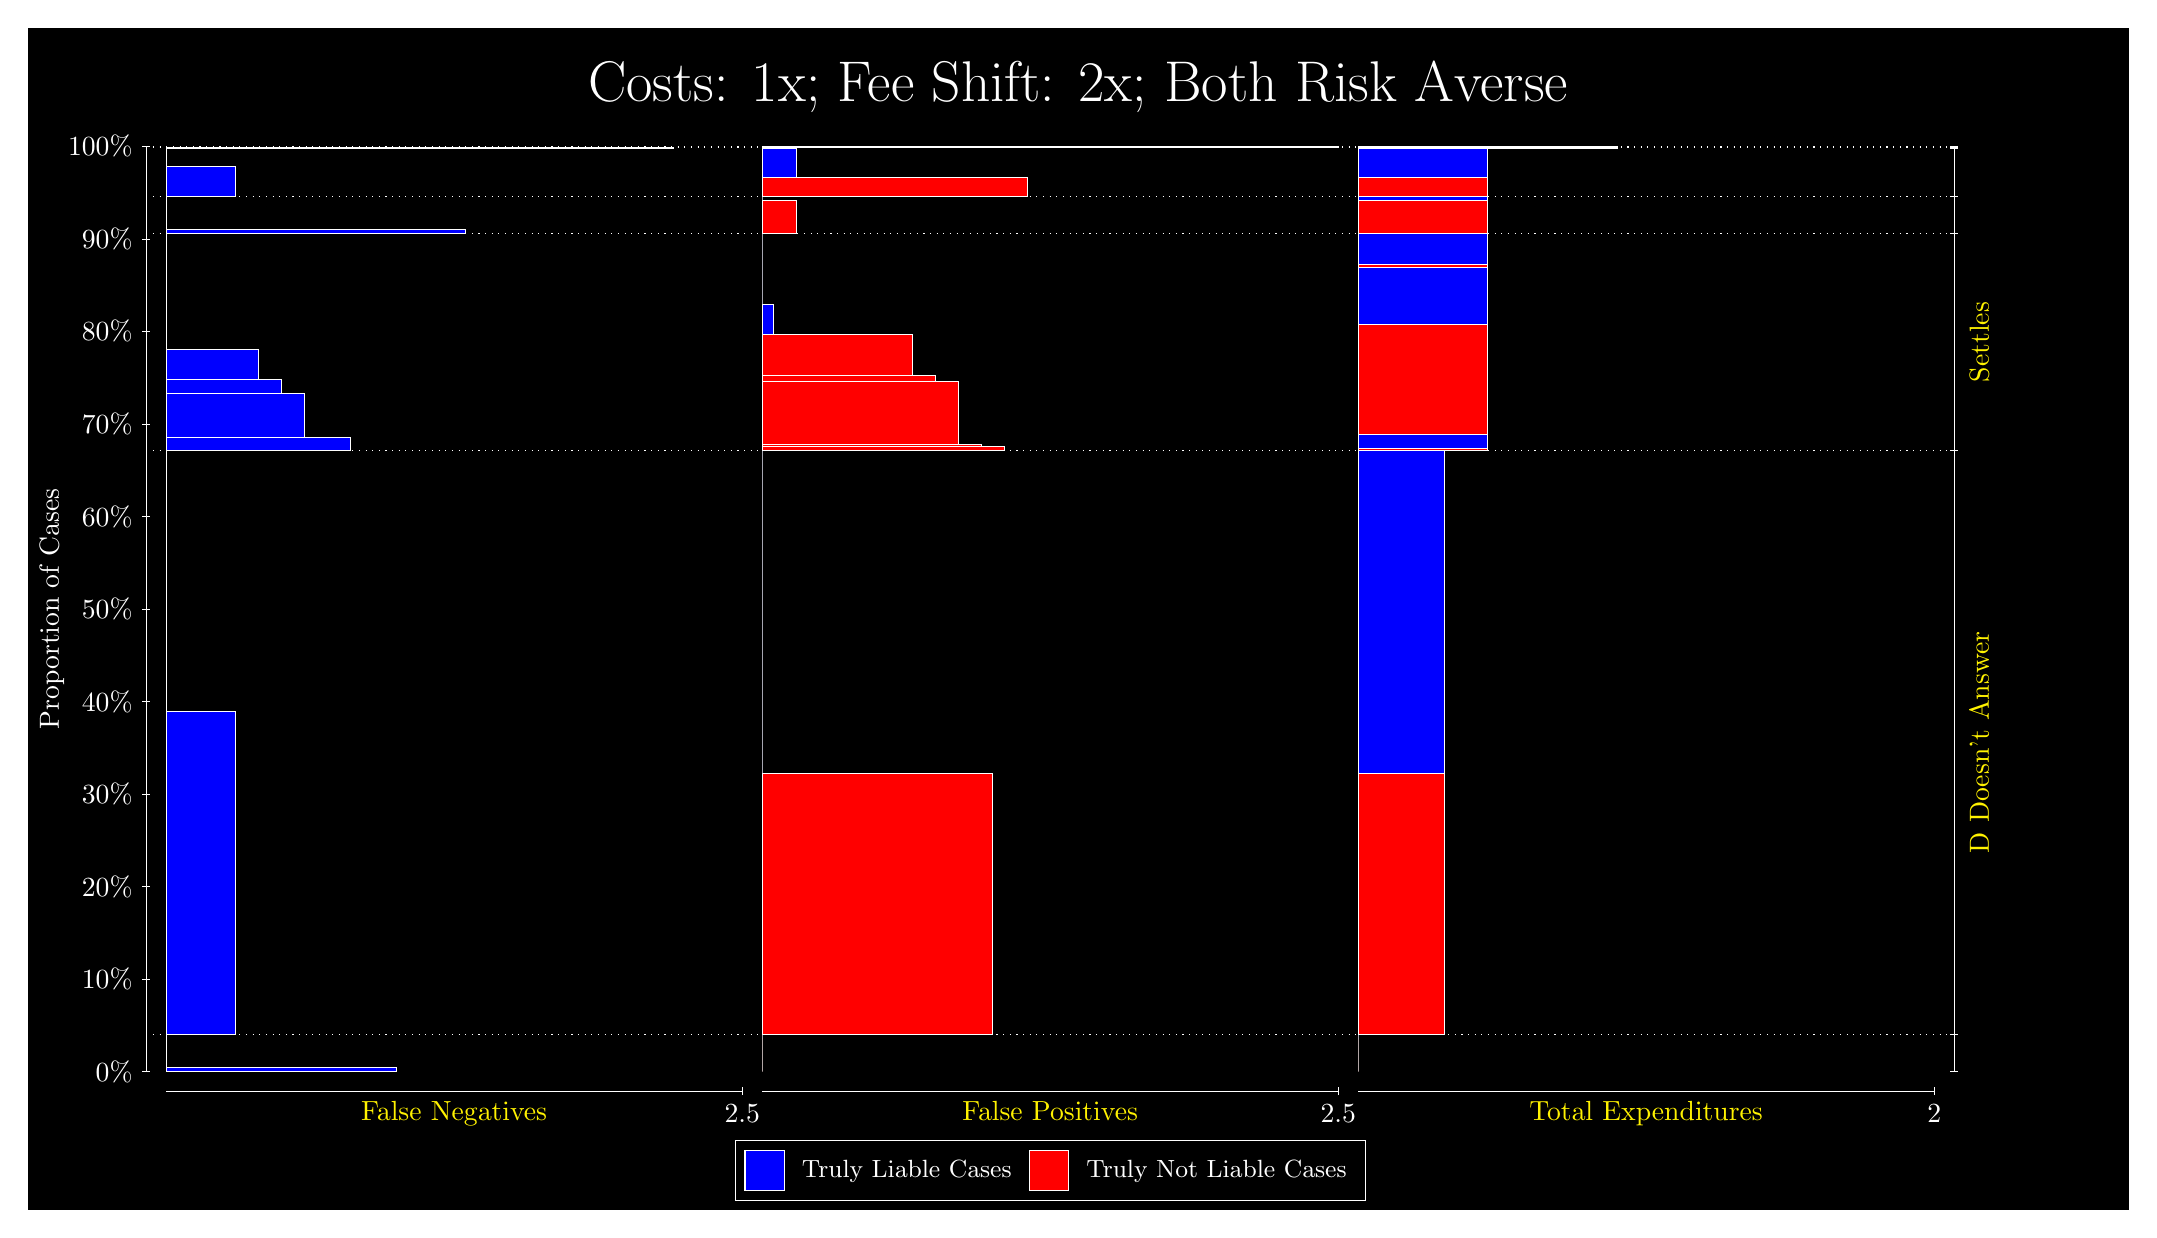
\begin{tikzpicture}
\draw[fill=black] (0,0) rectangle (26.667,15);
\draw[text=white] (0,13.5) rectangle (26.667,15) node[midway] {\huge Costs: 1x; Fee Shift: 2x; Both Risk Averse};
\draw[white, very thin] (1.5,1.75) -- (1.5,13.5);
\node[rotate=90, text=white, anchor=center] at (0.3, 7.625) {Proportion of Cases};
\draw[white, very thin] (1.45,1.75) -- (1.55,1.75);
\node[text=white, anchor=east] at (1.45, 1.75) {0\%};
\draw[white, very thin] (1.45,2.925) -- (1.55,2.925);
\node[text=white, anchor=east] at (1.45, 2.925) {10\%};
\draw[white, very thin] (1.45,4.1) -- (1.55,4.1);
\node[text=white, anchor=east] at (1.45, 4.1) {20\%};
\draw[white, very thin] (1.45,5.275) -- (1.55,5.275);
\node[text=white, anchor=east] at (1.45, 5.275) {30\%};
\draw[white, very thin] (1.45,6.45) -- (1.55,6.45);
\node[text=white, anchor=east] at (1.45, 6.45) {40\%};
\draw[white, very thin] (1.45,7.625) -- (1.55,7.625);
\node[text=white, anchor=east] at (1.45, 7.625) {50\%};
\draw[white, very thin] (1.45,8.8) -- (1.55,8.8);
\node[text=white, anchor=east] at (1.45, 8.8) {60\%};
\draw[white, very thin] (1.45,9.975) -- (1.55,9.975);
\node[text=white, anchor=east] at (1.45, 9.975) {70\%};
\draw[white, very thin] (1.45,11.15) -- (1.55,11.15);
\node[text=white, anchor=east] at (1.45, 11.15) {80\%};
\draw[white, very thin] (1.45,12.325) -- (1.55,12.325);
\node[text=white, anchor=east] at (1.45, 12.325) {90\%};
\draw[white, very thin] (1.45,13.5) -- (1.55,13.5);
\node[text=white, anchor=east] at (1.45, 13.5) {100\%};

\draw[white, very thin] (24.457,1.75) -- (24.457,13.5);
\draw[white, very thin] (24.407,1.75) -- (24.507,1.75);
\node[anchor=west] at (24.407, 1.75) {};
\draw[white, very thin] (24.407,2.2228) -- (24.507,2.2228);
\node[anchor=west] at (24.407, 2.2228) {};
\draw[white, very thin] (24.407,9.6394) -- (24.507,9.6394);
\node[anchor=west] at (24.407, 9.6394) {};
\draw[white, very thin] (24.407,12.391) -- (24.507,12.391);
\node[anchor=west] at (24.407, 12.391) {};
\draw[white, very thin] (24.407,12.868) -- (24.507,12.868);
\node[anchor=west] at (24.407, 12.868) {};
\draw[white, very thin] (24.407,13.481) -- (24.507,13.481);
\node[anchor=west] at (24.407, 13.481) {};
\draw[white, very thin] (24.407,13.494) -- (24.507,13.494);
\node[anchor=west] at (24.407, 13.494) {};
\draw[white, very thin] (24.407,13.5) -- (24.507,13.5);
\node[anchor=west] at (24.407, 13.5) {};

\draw[white, very thin, fill=blue] (1.75,1.75) rectangle (4.6775,1.7997);
\draw[white, very thin, fill=red] (1.75,1.7997) rectangle (1.75,2.2228);
\draw[white, very thin, fill=blue] (1.75,2.2228) rectangle (2.6283,6.3307);
\draw[white, very thin, fill=red] (1.75,6.3307) rectangle (1.75,9.6394);
\draw[white, very thin, fill=blue] (1.75,9.6394) rectangle (4.092,9.7999);
\draw[white, very thin, fill=blue] (1.75,9.7999) rectangle (3.7993,9.8065);
\draw[white, very thin, fill=blue] (1.75,9.8065) rectangle (3.5065,10.363);
\draw[white, very thin, fill=blue] (1.75,10.363) rectangle (3.2138,10.536);
\draw[white, very thin, fill=blue] (1.75,10.536) rectangle (2.921,10.92);
\draw[white, very thin, fill=red] (1.75,10.92) rectangle (1.75,12.391);
\draw[white, very thin, fill=blue] (1.75,12.391) rectangle (5.5558,12.444);
\draw[white, very thin, fill=red] (1.75,12.444) rectangle (1.75,12.868);
\draw[white, very thin, fill=blue] (1.75,12.868) rectangle (2.6283,13.245);
\draw[white, very thin, fill=red] (1.75,13.245) rectangle (1.75,13.481);
\draw[white, very thin, fill=blue] (1.75,13.481) rectangle (8.1906,13.484);
\draw[white, very thin, fill=red] (1.75,13.484) rectangle (1.75,13.494);
\draw[white, very thin, fill=red] (1.75,13.494) rectangle (1.75,13.497);
\draw[white, very thin, fill=blue] (1.75,13.497) rectangle (1.75,13.5);
\draw[white, very thin, fill=red] (9.3189,1.75) rectangle (9.3189,2.1731);
\draw[white, very thin, fill=blue] (9.3189,2.1731) rectangle (9.3189,2.2228);
\draw[white, very thin, fill=red] (9.3189,2.2228) rectangle (12.246,5.5315);
\draw[white, very thin, fill=blue] (9.3189,5.5315) rectangle (9.3189,9.6394);
\draw[white, very thin, fill=red] (9.3189,9.6394) rectangle (12.393,9.6864);
\draw[white, very thin, fill=red] (9.3189,9.6864) rectangle (12.1,9.7131);
\draw[white, very thin, fill=red] (9.3189,9.7131) rectangle (11.807,10.521);
\draw[white, very thin, fill=red] (9.3189,10.521) rectangle (11.515,10.593);
\draw[white, very thin, fill=red] (9.3189,10.593) rectangle (11.222,11.11);
\draw[white, very thin, fill=blue] (9.3189,11.11) rectangle (9.4652,11.494);
\draw[white, very thin, fill=blue] (9.3189,11.494) rectangle (9.3189,12.391);
\draw[white, very thin, fill=red] (9.3189,12.391) rectangle (9.758,12.815);
\draw[white, very thin, fill=blue] (9.3189,12.815) rectangle (9.3189,12.868);
\draw[white, very thin, fill=red] (9.3189,12.868) rectangle (12.686,13.104);
\draw[white, very thin, fill=blue] (9.3189,13.104) rectangle (9.758,13.481);
\draw[white, very thin, fill=red] (9.3189,13.481) rectangle (9.3189,13.491);
\draw[white, very thin, fill=blue] (9.3189,13.491) rectangle (9.3189,13.494);
\draw[white, very thin, fill=red] (9.3189,13.494) rectangle (16.638,13.497);
\draw[white, very thin, fill=blue] (9.3189,13.497) rectangle (13.71,13.5);
\draw[white, very thin, fill=red] (16.888,1.75) rectangle (16.888,2.1731);
\draw[white, very thin, fill=blue] (16.888,2.1731) rectangle (16.888,2.2228);
\draw[white, very thin, fill=red] (16.888,2.2228) rectangle (17.986,5.5315);
\draw[white, very thin, fill=blue] (16.888,5.5315) rectangle (17.986,9.6394);
\draw[white, very thin, fill=red] (16.888,9.6394) rectangle (18.534,9.6661);
\draw[white, very thin, fill=blue] (16.888,9.6661) rectangle (18.534,9.8391);
\draw[white, very thin, fill=red] (16.888,9.8391) rectangle (18.534,11.236);
\draw[white, very thin, fill=blue] (16.888,11.236) rectangle (18.534,11.96);
\draw[white, very thin, fill=red] (16.888,11.96) rectangle (18.534,12.007);
\draw[white, very thin, fill=blue] (16.888,12.007) rectangle (18.534,12.391);
\draw[white, very thin, fill=red] (16.888,12.391) rectangle (18.534,12.815);
\draw[white, very thin, fill=blue] (16.888,12.815) rectangle (18.534,12.868);
\draw[white, very thin, fill=red] (16.888,12.868) rectangle (18.534,13.104);
\draw[white, very thin, fill=blue] (16.888,13.104) rectangle (18.534,13.481);
\draw[white, very thin, fill=red] (16.888,13.481) rectangle (20.181,13.491);
\draw[white, very thin, fill=blue] (16.888,13.491) rectangle (20.181,13.494);
\draw[white, very thin, fill=red] (16.888,13.494) rectangle (20.181,13.497);
\draw[white, very thin, fill=blue] (16.888,13.497) rectangle (20.181,13.5);
\draw[white, dotted] (1.5,2.2228) -- (24.457,2.2228);
\draw[white, dotted] (1.5,9.6394) -- (24.457,9.6394);
\draw[white, dotted] (1.5,12.391) -- (24.457,12.391);
\draw[white, dotted] (1.5,12.868) -- (24.457,12.868);
\draw[white, dotted] (1.5,13.481) -- (24.457,13.481);
\draw[white, dotted] (1.5,13.494) -- (24.457,13.494);
\draw[white, very thin] (1.75,1.5) -- (9.0689,1.5);
\node[text=yellow, anchor=north] at (5.4094, 1.5) {False Negatives};
\draw[white, very thin] (9.0689,1.45) -- (9.0689,1.55);
\node[text=white, anchor=north] at (9.0689, 1.45) {2.5};

\draw[white, very thin] (9.3189,1.5) -- (16.638,1.5);
\node[text=yellow, anchor=north] at (12.978, 1.5) {False Positives};
\draw[white, very thin] (16.638,1.45) -- (16.638,1.55);
\node[text=white, anchor=north] at (16.638, 1.45) {2.5};

\draw[white, very thin] (16.888,1.5) -- (24.207,1.5);
\node[text=yellow, anchor=north] at (20.547, 1.5) {Total Expenditures};
\draw[white, very thin] (24.207,1.45) -- (24.207,1.55);
\node[text=white, anchor=north] at (24.207, 1.45) {2};


\node[text=yellow, centered, rotate=90] at (24.777, 5.9311) {D Doesn't Answer};
\node[text=yellow, centered, rotate=90] at (24.777, 11.015) {Settles};





\draw (12.978300999999998,1.5) node[draw=none] (baseCoordinate) {};
\begin{scope}[align=center]
        \matrix[scale=0.5, draw=white, below=0.5cm of baseCoordinate, nodes={draw}, column sep=0.1cm]{
            \node[rectangle, draw, minimum width=0.5cm, minimum height=0.5cm, fill=blue] {}; &
            \node[draw=none, font=\small, text=white] (B) {Truly Liable Cases}; &
            \node[rectangle, draw, minimum width=0.5cm, minimum height=0.5cm, fill=red] {}; &
            \node[draw=none, font=\small, text=white] (B) {Truly Not Liable Cases}; \\
            };
\end{scope}

\end{tikzpicture}
\end{document}